% A path homotopy F_s continuously deforming alpha (= F_0) to beta (= F_1)
% between two fixed endpoints p, q in the complex plane.
% Source: book/tex/topology/top-more.tex (§ Homotopy).
\documentclass[border=2mm]{standalone}
\usepackage{amssymb}
\usepackage{tikz}
\begin{document}
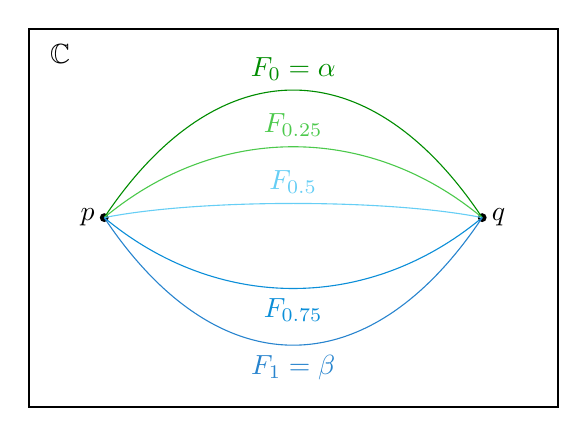
\begin{tikzpicture}[scale=0.8]
  \draw[black, line width=0.7pt] (-4.2,-3) rectangle (4.2,3);
  \node at (-3.7,2.6) {$\mathbb{C}$};
  \fill (-3,0) circle (2pt) node[left] {$p$};
  \fill (3,0) circle (2pt) node[right] {$q$};
  \draw[green!55!black] (-3,0) .. controls (-1.2,2.7) and (1.2,2.7) .. (3,0)
    node[pos=0.5, above] {$F_0=\alpha$};
  \draw[green!70!black!70] (-3,0) .. controls (-1.2,1.5) and (1.2,1.5) .. (3,0)
    node[pos=0.5, above] {$F_{0.25}$};
  \draw[cyan!60] (-3,0) .. controls (-1.5,0.3) and (1.5,0.3) .. (3,0)
    node[pos=0.5, above] {$F_{0.5}$};
  \draw[cyan!75!blue] (-3,0) .. controls (-1.2,-1.5) and (1.2,-1.5) .. (3,0)
    node[pos=0.5, below] {$F_{0.75}$};
  \draw[cyan!60!blue!90] (-3,0) .. controls (-1.2,-2.7) and (1.2,-2.7) .. (3,0)
    node[pos=0.5, below] {$F_1=\beta$};
\end{tikzpicture}
\end{document}
